\chapter{Results}


This section describes the results of refactoring pyProCT with pyCOMPSs. I divided into three subsections. The first one reports the benefits of using pyCOMPSs programming model. The second subsection contains the performance analysis of the results. Finally, the last part deals with tools that the framework offers.

\section{Programming Model}

pyCOMPSs framework is supposed to require little extra code to be used so first I will compare difference of size between each version. Figure \ref{tab:sizes} shows the comparison between the different classes required. It's based on the number of characters and lines because python conventions encourage the usage of line breaks so the results could be misleading (some functions have one parameter per line).


\begin{center}
	\begin{tabular}{| R{6cm} | L{3cm} | L{3cm} |}
		\hline
		Class Name & Original & pyCOMPSs \\ 
		\hline
		\hline
		Driver & 169 / 8180  &  165 / 7911 \\
		\hline
		ClusteringProtocol & 78 / 3703 & 73 / 3490 \\
		\hline
		PostProcessingDriver & 32 / 1531 & 56 / 2700 \\
		\hline
		ClusteringExplorer & 195 / 8470 & 197 / 9226 \\ 
		\hline
	\end{tabular}
	\captionof{table}{Size comparison of duplicated classes} 
	\label{tab:sizes}
\end{center}


We see that the refactor did not add too much space. The driver and protocol classes are in fact shorter. This is caused because of the removal of the task-adding loop and the pyScheduler initialization. Postprocessing driver is longer due to the fact that on the original version this section is not parallel. The other ones are quite even.

PyCOMPSs framework just uses python decorators and API calls so, why do we observe a size increase in some classes? This is due to the fact that our data can not automatically serialized by python's pickle. Almost all the extra size is linked to the work needed to handle the matrix data. However, other than adding this little size overhead, the code is much clean and easy to read. 

Another important aspect is the execution process and tools offered by the framework. It is here were COMPSs truly shines. 

The level of hardware abstraction provided by the framework is really good. To execute pyProCT in a local environment one just needs to provide the language (python on this case), classpath, executable and parameters. If the user desires to customize the framework offers two kind of hardware configurations. On the one hand we find the \textit{resources.xml}. This file allows to define the workers to be used. This includes supercomputer nodes, cloud services, remote images and more. On the other hand we have the \textit{project.xml} which selects which of the defined resources are to be actually used and some runtime parameters. 

With this simple two files we can define a wide range of available resources to be used and then select which ones we want to use for an specific execution. Thanks to this we can use a lot of different resources without worrying about the internals and communications. COMPSs' already implements all the connectors required to use them so we just need to give a description of them, select which to use and decorate our code. 

For MareNostrum III executions this process is even easier. The development team has created scripts to submit jobs to the supercomputer. By default, it requires the same parameters as a normal execution. However, it has a wide range of easy-to-use options with a clear description. With all the parameters available, such as the network and file system to be used or the number of nodes, it automatically creates the \textit{resources.xml} and \textit{project.xml} that best suit our needs. 

This is tools are really useful. Most of the time working of this project has been spent on trying to execute the program on the supercomputer. One needs to understand how a submission queue system works, which parameters need to be specified, how the class paths are read and used, which way the supercomputer access files, which kind of problems may arise from mutex access to the datasets and so on. This is a quite daunting task for someone without advanced knowledge on the subject or with no one to ask help to. 

As stated, COMPSs required number of parameters are far less. Understanding some of the aforementioned things will help the user to better use the framework but they are not really mandatory because the COMPSs manuals are good and clear. Following the examples is enough to execute your own programs. 




\section{Performance}

\label{sec:resperformance}

This section reports the results of the refactor related with the performance. 

Throughout this section some traces will be presented to describe the numerical results. However, the times reported on the traces can not be compared. This is due to the fact that each parallelization is instrumented with a different method (see Appendix \ref{sec:instrumentation}). Because of that we can not trust the reported times; pyCOMPSs and multiprocessing instrumentation are far slower than the MPI version because they need to create a process to emit each of the events.

When reporting execution times the x-axis will frequently contain number of threads/processes used. However, when queueing pyCOMPSs executions we specify the desired amount of nodes being the minimum 2 (one is used for the runtime/master which handles all the framework). For this reason, the executions will start at 32 processes/threads which corresponds to that 2 nodes (each node uses 16 threads). Instead, for multiprocessing the execution will be limited to 16 because it can not run on more than one node.


The following datasets will be used:

\begin{itemize}
%TODO add datasets used
\item
\end{itemize}

COMPSs is designed to harness all the power of supercomputers and use all the available computing resources. The whole initialization of such a framework is not a trivial matter and because of that I expect it to be slow with respect to MPI or OpenMP. However, being designed to run programs with humongous datasets and computation times, this initial overhead is negligible. I expect to see that MPI and multiprocessing schedulers are faster than pyCOMPSs on small datasets and slower on larger ones. 

Figure \ref{fig:small} shows that indeed COMPSs is the slowest parallelization for the smallest dataset. We can observe that multiprocessing is the fastest. That is caused because this method is only able to work on a single node so the initialization and overhead of data and resources handling is indeed much smaller.

\begin{figure}[h]
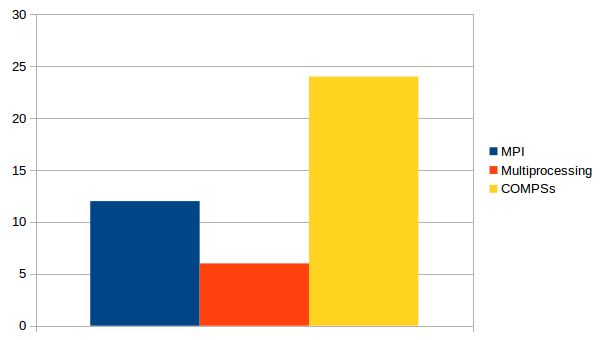
\includegraphics[width=\textwidth]{img/small_graphs.png}
\caption{Execution times on small dataset given the number of threads}
\label{fig:small}
\end{figure}

We can observe that the execution time of each parallelization increases or is stable with the number of threads instead of decrease. COMPSs decrease with 48 processes is not significant as the variance is of just one second. In order to see why the executions are stable we will have a look at the traces to see if it is a task allocation problem.

Figure \ref{tra:par16small} shows the trace for multiprocessing execution with 16 threads. The code is intrumented following pyProCT structure: initialization and parameters handling, data, clustering and postprocess. First blue stripe is the time from the start till the data section. The white one is the matrix handling and calculation. After that all the red section is the actual clustering and analysis. Last strip of first thread is the postprocess. The purple sections correspond to the algorithms and analysis tasks. Note that for multiprocessing the first thread also performs task but they are not shown because we preferred to mark the clustering section. Note that execution is sequential until the program reaches the clustering section where it uses the parallel scheduler. We can also observer that all tasks are equally distributed amongst all the available threads. 

\begin{figure}[h]
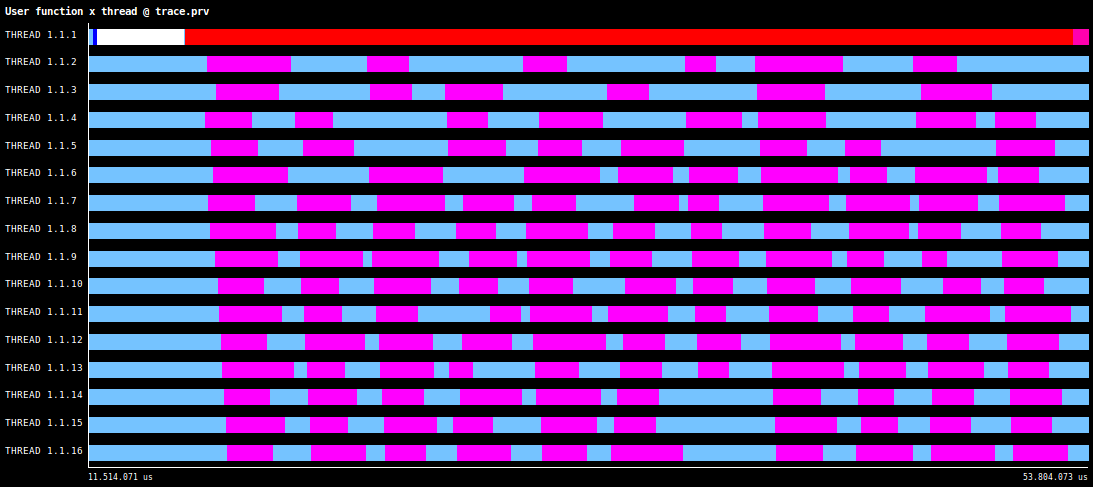
\includegraphics[width=\textwidth]{traces/par_16_small.png}
\caption{Multiprocessing scheduler with small dataset and 16 threads}
\label{tra:par16small}
\end{figure}

Next, figure \ref{tra:mpi16small} shows the same execution but with the MPI scheduler. First is important to see that the all the data section (in purple) and thus the matrix calculation is performed on all the threads. MPI scheduler handles the available pool of threads just when they reach the actual scheduler. That means that all the threads are doing the same work till that point and so it's redundant work. Despite that, the postprocessing section (in red) does take into the available pool and uses just one thread to avoid work duplication. 

White section is the clustering section. Inside, the green parts are the ones adding the tasks to the scheduler and the blues the actual algorithms execution. The blue stripes outside the white part are the ones corresponding to the analysis tasks (which have the same name and thus the same color).Even if all the threads are performing the task-adding loop they are added only once because the task's name must be unique. Please note that blue stripes are composed of a lot of littler ones (the number of tasks is the same on both executions)  

We can see that on MPI the matrix calculation is quite longer than the multiprocessing (with respect to its own total time as we can not compare across traces). This is because having 16 threads busy makes them all go slower because, being in the same node, they share some resources (like cache) and all of them are accessing the same input file. On the loop that adds the tasks we see again the same behaviour: duplicated work that wastes resources and increases execution time. 

Comparing the two traces we see that multiprocessing is almost all the time in parallel mode and that the sequential parts are small. MPI, on the other hand, despite running in parallel almost all the time it just does useful work in the blue stripes. However, multiprocessing is limited to 16 threads so this is it's performance peak and MPI can use more resources.

\begin{figure}[h]
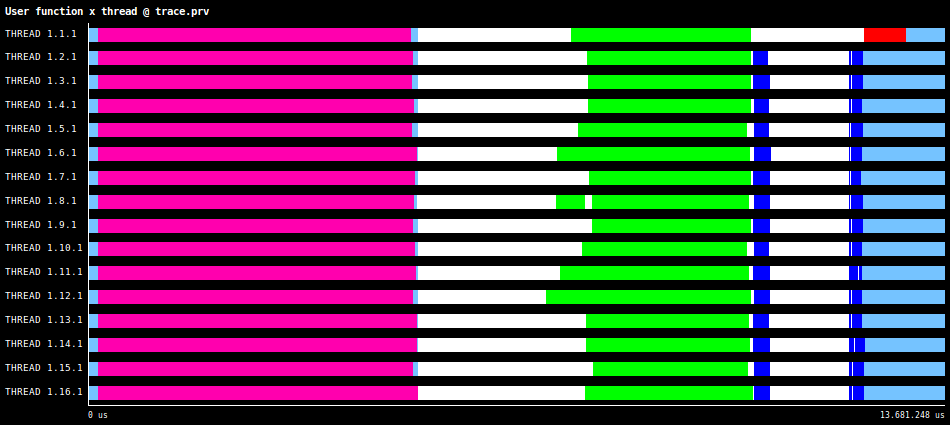
\includegraphics[width=\textwidth]{traces/mpi_16_small.png}
\caption{MPI scheduler with small dataset and 16 threads}
\label{tra:mpi16small}
\end{figure}

\section{Tools}